\section{Mortal Kombat Armageddon}

\begin{figure}[htbp]
\begin{center}
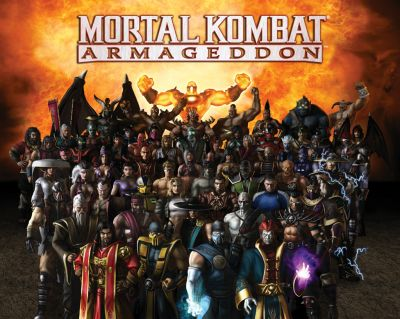
\includegraphics[width=.60\textwidth]{./imagenes/MortalK.jpg}
\caption{Mortal Kombat Armageddon}
\label{Mortal Kombat Armageddon}
\end{center}
\end{figure}

Mortal Kombat: Armageddon \footnote{\url{http://www.mortalkombat.net/armageddon/}} es un videojuego de la saga Mortal Kombat desarrollada por Midway Games. Este juego es una continuación directa de Mortal Kombat: Deception. El juego distribuyo más de 2 millones de copias por todo el mundo.
Las plataformas designadas para este juego son PlayStation 2 y Xbox en el 2006 y Wii en el 2007.

\subsubsection{¿Por qué es uno de mis juegos favoritos?}
\begin{itemize}
\item[Joao Sanga] Me gusta mucho por los gráficos, el modo de pelea y la historia. Las peleas en Mortal Kombat siempre conservarán su puntito gore (sangriento): sin él, nada diferenciaría a la saga de otros tantos juegos de lucha.
Aprendiendo de la experiencia en títulos pasados, MK Armageddon ha suavizado los controles, y ha ordenado todos los elementos en un sencillo menú. Pero la mecánica del juego sigue siendo la misma: cada luchador tiene dos métodos de combate –una técnica cuerpo a cuerpo, y lucha con arma-, junto con los clásicos combos aéreos, encadenados, llaves y contras. Quienes busquen un título de machaque fácil pulsando botones a toda velocidad, lo tienen complicado de nuevo: en Mortal Kombat los combates no lo parecen, SON lentos, ni de lejos tan vertiginosos como en cualquier juego de lucha de Namco. Los kombatientes se mueven en ocasiones como marionetas que responden mecánicamente a nuestras teclas.
En conclusión, Mortal Kombat Armageddon es uno de los mejores creados de la saga de Mortal Kombat.
\end{itemize}